\fenicschapter{Finite Element Assembly}
              {Finite Element Assembly}
              {Anders Logg, Kent-Andre Mardal and Garth N. Wells}
              {logg-3}

The finite element method may be viewed as a method for forming a
discrete linear system $AU = b$ or nonlinear system $b(U) = 0$
corresponding to the discretization of the variational form of a
differential equation. A central part of the implementation of finite
element methods is therefore the computation of matrices and vectors
from variational forms. In this chapter, we describe the standard
algorithm for computing the discrete operator (tensor) $A$ defined in
Chapter~[kirby-5]. This algorithm is known as finite element
assembly. We also discuss efficiency aspects of the standard algorithm
and extensions to matrix-free methods.

%------------------------------------------------------------------------------
\section{Assembly Algorithm}

The discrete operator~$A$ for a multilinear form~$a : V^1 \times
V^2 \times \cdots \times V^{\rho} \rightarrow \R$ of arity~$\rho$ is
the rank~$\rho$ tensor defined by
\begin{displaymath}
  A_i = a(\phi^1_{i_1}, \phi^2_{i_2}, \ldots, \phi^{\rho}_{i_{\rho}}),
\end{displaymath}
where $i = (i_1, i_2, \ldots, i_{\rho})$ is a multi-index of
length~$\rho$ and $\{\phi^j_i\}_{i=1}^{N_j}$ is a basis for $V^j_h
\subset V^j$, $j = 1,2,\ldots,\rho$. The discrete operator is a
typically sparse tensor of rank~$\rho$ and dimension $N_1 \times N_2
\times \cdots \times N_{\rho}$.
Details of the discrete operator~$A$ are provided in
Chapter~[kirby-5].

A straightforward algorithm to compute the tensor~$A$ is to iterate
over all its entries and compute the entries one at a time, as
outlined in Algorithm~\ref{alg:assembly,naive}.  This algorithm has
two major drawbacks and is rarely used in practice. First, it does not
take into account that most entries of the sparse tensor~$A$ may be
zero. Second, it does not take into account that each entry is
typically a sum of contributions (integrals) from the set of cells
that form the support of the basis functions
$\phi^1_{i_1}, \phi^2_{i_2}, \ldots,
\phi^{\rho}_{i_\rho}$. As a result, each cell of the mesh must be
visited multiple times when computing the local contribution to
different entries of the tensor~$A$.  For this reason, the tensor~$A$
is usually computed by iterating over the cells of the mesh and adding
the contribution from each local cell to the global tensor~$A$. To see
how the tensor~$A$ can be decomposed as a sum of local contributions,
we recall the definition of the cell tensor~$A_T$ from
Chapter~[kirby-5],
\begin{displaymath}
  A_{T,i} = a_T(\phi^{T,1}_{i_1}, \phi^{T,2}_{i_2}, \ldots, \phi^{T,\rho}_{i_{\rho}}),
\end{displaymath}
where $a_T$ is the local contribution to the multilinear form from a
cell~$T\in\mathcal{T}$ and $\{\phi^{T,j}_i\}_{i=1}^{n_j}$ is the local
finite element basis for $V^j_h$ on~$T$. We assume here that the
multilinear form is expressed as an integral over the domain~$\Omega$
so that it may be naturally decomposed as a sum of local
contributions. If the form contains contributions from facet or
boundary integrals, one may similarly decompose the multilinear form
into local contributions from facets.

\begin{algorithm}
  \begin{tabbing}
    \textbf{for} {$i_1 = 1,2,\ldots,N_1$}\\
    \tab \textbf{for} {$i_2 = 1,2,\ldots,N_2$}\\
    \tab \tab \textbf{for} \ldots \\
    \tab \tab \tab $A_i = a(\phi^1_i, \phi^2_j, \ldots, \phi^{\rho}_{i_{\rho}})$
  \end{tabbing}
  \caption{Straightforward (naive) ``assembly'' algorithm.}
  \label{alg:assembly,naive}
\end{algorithm}

To formulate the general assembly algorithm, let $\iota_T^j : [1,n_j]
\rightarrow [1,N_j]$ denote the local-to-global mapping introduced in
Chapter~[kirby-7] for each discrete function space $V^j_h$,
$j=1,2,\ldots,\rho$, and define for each $T \in \mathcal{T}$ the
collective local-to-global mapping $\iota_T : \mathcal{I}_T
\rightarrow \mathcal{I}$ by
\begin{equation}
  \iota_T(i) =
  (\iota_T^1(i_1),\iota_T^2(i_2),\ldots,\iota_T^{\rho}(i_{\rho}))
  \quad \forall i \in \mathcal{I}_T,
\end{equation}
where $\mathcal{I}_T$ is the index set
\begin{equation}
  \mathcal{I}_T =
  \prod_{j=1}^{\rho}[1,n_j] = \{(1,1,\ldots,1), (1,1,\ldots,2), \ldots,
  (n_1, n_2, \ldots, n_{\rho})\}.
\end{equation}
That is, $\iota_T$ maps a tuple of local degrees of freedom to a tuple
of global degrees of freedom. Furthermore, let $\mathcal{T}_i \subset
\mathcal{T}$ denote the subset of the mesh on which
$\{\phi_{i_j}^j\}_{j=1}^{\rho}$ are all nonzero. We note that
$\iota_T$ is invertible if $T \in \mathcal{T}_i$.
We may now compute the tensor~$A$ by summing local contributions from
the cells of the mesh,
\begin{equation}
  \begin{split}
  A_i
  &=
  \sum_{T\in\mathcal{T}}
  a_T(\phi_{i_1}^1, \phi_{i_2}^2, \ldots, \phi_{i_{\rho}}^{\rho})
  =
  \sum_{T\in\mathcal{T}_i}
  a_T(\phi_{i_1}^1, \phi_{i_2}^2, \ldots, \phi_{i_{\rho}}^{\rho}) \\
  &=
  \sum_{T\in\mathcal{T}_i}
  a_T(\phi_{(\iota_T^1)^{-1}(i_1)}^{T,1},
      \phi_{(\iota_T^2)^{-1}(i_2)}^{T,2}, \ldots,
      \phi_{(\iota_T^{\rho})^{-1}(i_{\rho})}^{T,{\rho}})
  =
  \sum_{T\in\mathcal{T}_i}
  A_{T,{\iota_T^{-1}(i)}}.
  \end{split}
\end{equation}
This computation may be carried out efficiently by a single iteration
over all cells~$T \in \mathcal{T}$. On each cell, the element
tensor~$A_T$ is computed and then added to the global tensor~$A$ as
outlined in Algorithm~\ref{alg:assembly} and illustrated in
Figure~\ref{fig:insertion}.
\begin{algorithm}
  \begin{tabbing}
    $A = 0$\\
    \textbf{for}  {$T \in \mathcal{T}$}\\
    \tab (1) Compute $\iota_T$ \\
    \tab (2) Compute $A_T$ \\ \\
    \tab (3) Add $A_T$ to $A$ according to $\iota_T$: \\
    \tab \textbf{for} $i \in \mathcal{I}_T$ \\
    \tab \tab $A_{\iota_T(i)} \stackrel{+}{=} A_{T,i}$ \\
    \tab \textbf{end for} \\
    \textbf{end for}
  \end{tabbing}
  \caption{Assembly algorithm}
  \label{alg:assembly}
\end{algorithm}

\begin{figure}
  \begin{center}
    %\psfrag{i0}{\hspace{-0.5cm}$\iota_T^1(1)$}
    %\psfrag{i1}{\hspace{-0.5cm}$\iota_T^1(2)$}
    %\psfrag{i2}{\hspace{-0.5cm}$\iota_T^1(3)$}
    %\psfrag{j0}{\hspace{-0.3cm}$\iota_T^2(1)$}
    %\psfrag{j1}{\hspace{-0.5cm}$\iota_T^2(2)$}
    %\psfrag{j2}{\hspace{-0.1cm}$\iota_T^2(3)$}
    %\psfrag{A21}{$A_{T,32}$}
    %\psfrag{1}{$1$}
    %\psfrag{2}{$2$}
    %\psfrag{3}{$3$}
    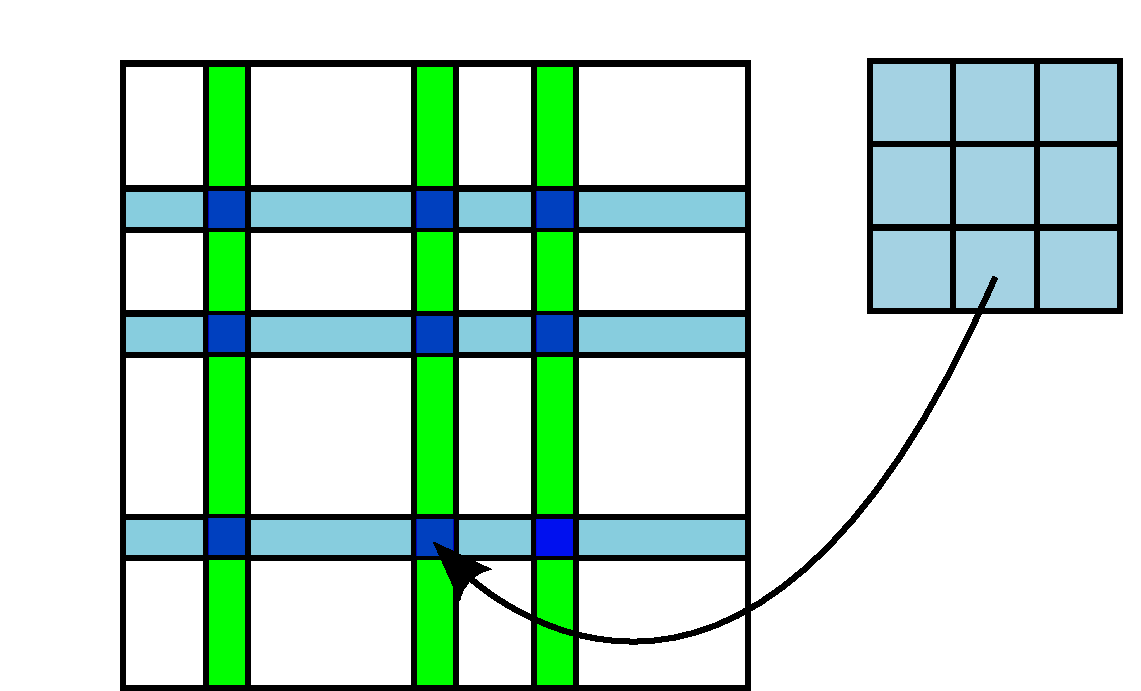
\includegraphics[width=12cm]{chapters/logg-3/pdf/insertion.pdf}
    \caption{Adding the entries of the element tensor~$A_T$ to the
      global tensor~$A$ using the  local-to-global mapping
      $\iota_T$, illustrated here for a rank two
      tensor (a matrix).}
    \label{fig:insertion}
  \end{center}
\end{figure}

%------------------------------------------------------------------------------
\section{Implementation}

In FEniCS, the assembly algorithm (Algorithm~\ref{alg:assembly}) is
implemented as part of DOLFIN (see
Figure~\ref{fig:assembly,code}). For the steps (1), (2) and (3) of the
assembly algorithm, DOLFIN relies on external code. For steps (1) and
(2), DOLFIN calls code generated by a form compiler such as FFC or
SyFi. In particular, DOLFIN calls the two
functions \emp{tabulate\_dofs} and
\emp{tabulate\_tensor} through the UFC interface for steps (1) and (2),
respectively. Step (3) is carried out through the DOLFIN
\emp{GenericTensor::add} interface and maps to the corresponding
operation in one of a number of linear algebra backends.
%For the two
%main linear algebra backends of FEniCS, which are
%PETSc~\cite{www:PETSc,BalBus04,BalEij97} and
%Trilinos/Epetra~\cite{trilinosreferences}, step (3) is mapped to
%\emp{MatSetValues} and \emp{SumInto\-Global\-Values} respectively.
%
\begin{figure}
  \begin{code}
for (CellIterator cell(mesh); !cell.end(); ++cell)
{
  ...

  // Tabulate dofs for each dimension
  for (uint i = 0; i < ufc.form.rank(); i++)
    a.function_space(i)->dofmap().tabulate_dofs(ufc.dofs[i],
                                                ufc.cell,
                                                cell->index());

  // Tabulate cell tensor
  integral->tabulate_tensor(ufc.A.get(), ufc.w, ufc.cell);

  // Add entries to global tensor
  if (values && ufc.form.rank() == 0)
    (*values)[cell->index()] = ufc.A[0];
  else
  {
    // Get local dimensions
    for (uint i = 0; i < ufc.form.rank(); i++)
      ufc.local_dimensions[i] =
        a.function_space(i)->dofmap().local_dimension(ufc.cell);
    A.add(ufc.A.get(), ufc.local_dimensions.get(), ufc.dofs);
  }

  ...
}
\end{code}
  \label{fig:assembly,code}
  \caption{Actual implementation (excerpt) of the assembly algorithm
    (Algorithm~\ref{alg:assembly}) in DOLFIN (from \emp{Assembler.cpp}
    in DOLFIN~0.9.7).}
\end{figure}

In typical assembly implementations, step (2), the computation of the
element tensor~$A_T$, is the most costly operation of the assembly
algorithm. For \dolfin{}, however, as a result of optimized algorithms
for the computation of $A_T$ being generated by form compilers (see
Chapters~[oelgaard-2] and~[kirby-8]), adding entries in
the local tensor $A_T$ to appropriate positions in the global
tensor~$A$ often constitutes a significant portion of the total assembly
cost. This operation is costly since the addition of a value to an
arbitrary entry of a sparse tensor is not a trivial operation, even when
the layout of the sparse matrix has been initialized.  In the standard
case when $A$ is a sparse matrix (a rank two tensor), the linear
algebra backend stores the sparse matrix in compressed row storage
(CRS) format or some other sparse format. For each given entry, the
linear algebra backend must search along a row~$i$ to find the
position to store the value for a given column~$j$. As a result, the
speed of assembly in FEniCS for sparse matrices is currently limited
by the speed of insertion into a sparse linear algebra data
structure. An additional cost is associated with the initialization of
a sparse matrix, which involves the computation of a sparsity
pattern. For most linear algebra libraries, it is necessary to
initialize the layout of a sparse matrix before inserting entries in
order to achieve tolerable insertion speed.  Computation of the
sparsity pattern is a moderately costly operation, but which in the
case nonlinear problems is usually amortized over time.

Algorithm~\ref{alg:assembly} may be easily extended to assembly over
the facets of a mesh. Assembly over facets is necessary both for
handling variational forms that contain integrals over the boundary of
a mesh (the exterior facets), to account for Neumann boundary
conditions, and forms that contain integrals over the interior facets
of a mesh as part of a discontinuous Galerkin formulation. For this
reason, DOLFIN implements three different assembly algorithms. These
are assembly over cells, exterior facets and interior facets.

%------------------------------------------------------------------------------
\section{Symmetric Application of Boundary Conditions}

For symmetric problems, it is useful to be able to apply Dirichlet
boundary conditions in a fashion that preserves the symmetry of the
matrix, since that allows solution algorithms which are limited to
symmetric matrices, such as the conjugate gradient method and Cholesky
decomposition, to be applied.  The symmetric application of boundary
conditions may be handled by modifying element tensors $A_T$ before
assembly into the global tensor~$A$.
%It involves computing both the local matrix and vector, and the
%applying partial Gauss elimination to incorporate the boundary
%condition.
Assembly with the symmetric application of boundary conditions is
implemented in DOLFIN in the class \emp{SystemAssembler}.
%This
%function assembles the complete linear system including boundary
%conditions.

To explain the symmetric assembly algorithm, consider the global
system $AU=b$ and the corresponding element matrix $A_T$ and
element vector~$b_T$. If a global index $i$ is associated with a
Dirichlet boundary condition, $U_i=D_i$, then this condition can be
enforced by setting $A_{ii} = 1$, $A_{ij} = 0$ for $i \neq j$, and
$b_i = D_i$. This approach is applied when calling the DOLFIN
function \emp{DirichetBC::apply}. However, to preserve symmetry of the
matrix, we can perform a partial Gaussian elimination to obtain
$A_{ji} = A_{ij} = 0$ for $i \ne j$.  This is achieved by subtracting
the $i$th row multiplied by $A_{ji}$ from the $j$th equation,
locally. These partial Gaussian eliminations are performed on the
linear systems at the element level. The local linear systems are then
added to the global matrix. As a result, the Dirichlet condition is
added multiple times to the global vector, one time for each cell,
which is compensated for by the addition of one multiple times to the
corresponding diagonal entry of~$A$ This algorithm is summarized in
Algorithm~\ref{alg:assembly:sym}. The described algorithm does not
eliminate the degrees of freedom associated with a Dirichlet boundary
condition from the global linear system, although it is possible to do
so. The `Dirichlet' degrees of freedom are retained to preserve the
integrity of any finite element functions which are represented in
terms of the degrees of freedom.
%It is possible to eliminate the degrees of freedom and insert the
%Dirichlet values when representing a finite element function, but this
%would increase the complexity of the necessary code.

\begin{algorithm}
  \begin{tabbing}
    $A = 0$ and $b = 0$\\\
    \textbf{for}  {$T \in \mathcal{T}$}\\
    \tab (1) Compute $\iota^A_T$ and $\iota^b_T$  \\
    \tab (2) Compute $A_T$ and $b_T$ \\
    \tab (3) Apply Dirichlet boundary conditions to $A_T$ and $b_T$ \\
    \tab (4) Perform partial Gaussian elimination on $A_T$ and $b_T$ to preserve symmetry \\
    \tab (5) Add $A_T$ and $b_T$ to $A$ and $b$ according to $\iota^A_T$ and $\iota^b_T$, respectively: \\
    \tab \textbf{for} $(i,j) \in \mathcal{I}^A_T$ \\
    \tab \tab $A_{\iota^{A,1}_T(i), \iota^{A,2}_T(j)} \stackrel{+}{=} A_{T,ij}$ \\
    \tab \textbf{end for} \\
    \tab \textbf{for} $i \in \mathcal{I}^b_T$  \\
    \tab \tab $b_{\iota^b_T(i)} \stackrel{+}{=} b^K_i$  \\
    \tab \textbf{end for} \\
    \textbf{end for}
  \end{tabbing}
  \label{alg:assembly:sym}
  \caption{Symmetric assembly algorithm}
\end{algorithm}

%------------------------------------------------------------------------------
\section{Parallel Assembly}

The assembly algorithms remain unchanged in a distributed parallel
environment if the linear algebra backend supports distributed
matrices and insertion for both on- and off-process matrix entries,
and if the mesh data structure supports distributed meshes. Both
PETSc~\cite{BalayBuschelmanGroppEtAl2001,BalayBuschelmanEtAl2004} and
Trilinos/Epetra~\cite{HerouxBartlettHowleEtAl2005} support distributed
matrices and vectors. Efficient parallel assembly relies on
appropriately partitioned meshes and properly distributed
degree-of-freedom maps to minimize inter-process communication.  It is
not generally possible to produce an effective degree-of-freedom map
using only a form compiler, since the degree-of-freedom map should
reflect the partitioning of the mesh. Instead, one may use a
degree-of-freedom map generated by a form compiler to construct a
suitable map at run-time.
\dolfin{} supports distributes meshes and computes distributed
degree of freedom maps for distributed assembly.

Multi-threaded assembly is outwardly simpler than distributed assembly
and is attractive given the rapid growth in multi-core architectures.
The assembly code can be easily modified, using for example OpenMP,
to parallelize
the assembly loop over cells.  However, multi-threaded assembly is
problematic at present since few linear algebra backends provide
thread-safe insertion. It is likely that future linear algebra
libraries will support a mixture of the distributed and multi-threaded
paradigms.

%------------------------------------------------------------------------------
\section{Matrix-Free Methods}

A feature of Krylov subspace methods and some other iterative methods
for linear systems of the form $AU = b$ is that they rely only on
the \emph{action} of the matrix operator $A$ on a vector and do not
require direct manipulation of~$A$. This is in contrast with direct
linear solvers. Therefore, if the action of $A$ on a vector $v$ can be
computed, then a Krylov solver can be used to solve the system $AU =
b$ without needing to assemble~$A$. This matrix-free approach may be
attractive for problem types which are well-suited to Krylov solvers
and for which the assembly of $A$ is costly (in terms of CPU time
and/or memory).  A disadvantage of matrix-free methods is that the
preconditioners that are most commonly used to improve the convergence
properties and robustness of Krylov solvers do involve manipulations
of $A$; hence these cannot be applied in a matrix-free approach. For
the purpose of assembly, a matrix-free approach replaces the assembly
of the matrix $A$ with repeated assembly of a vector $Av$, which is
the action of $A$ on the given vector~$v$. A key element in the
efficient application of such methods is the rapid assembly of
vectors. Insertion costs for dense vectors are relatively low, with
the computation of element contributions the dominant cost. Both
DOLFIN and the form compilers available as part of FEniCS support
assembly of the action of linear or linearized operators.
